\section{Design process}
\subsection{Analog}
The analog part of the circuit was designed and verified using SPICE simulations in  AIM-SPICE. 
As the device models where provided, the task was to develop the SPICE nets and simulation stimuli.\\
To allow a low voltage drop over the transistors, the length of the NMOS transistors where picked to be as short as possible, while maintaining the project specification, as shown in \cref{tab:trans}. 
The width of the NMOS was therefore picked as wide possible. 
The PMOS transistors where picked to be equally as strong as the NMOS transistors. 
Therefore the PMOS lengths where picked to be equal, but the widths should be slightly larger due to the mobility relation between the transistors.

\begin{table}[!htbp]
    \centering
    \begin{tabular}{c|c|c}
        Transistor & L  & W \\\hline
        M1 & \SI{0.40}{\micro\meter} & \SI{1.20}{\micro\meter} \\
        M2 & \SI{0.40}{\micro\meter} & \SI{1.20}{\micro\meter} \\
        M3 & \SI{0.40}{\micro\meter} & \SI{4.63}{\micro\meter} \\ 
        M4 & \SI{0.40}{\micro\meter} & \SI{4.63}{\micro\meter}
    \end{tabular}
    \caption{Transistor dimension specifications}
    \label{tab:trans}
\end{table}

As both CC1 and CC2 where given, the only capacitor that had to be chosen was CS. The value of CS was picked to be large enough to be charged during exposure, as well as not being to large as that would reduce the speed of operation. Capacitor values are shown in \cref{tab:caps}.

\begin{table}[!htbp]
    \centering
    \begin{tabular}{c|c}
        Capacitor & Capacitance \\\hline
        CS  & \SI{2}{\pico\farad} \\
        CC1 & \SI{3}{\pico\farad} \\
        CC2 & \SI{3}{\pico\farad}
    \end{tabular}
    \caption{Capacitor specifications}
    \label{tab:caps}
\end{table}

\subsubsection{Corner analysis}
\label{Corn_analysis}
To demonstrate process variation, a simulation for an NMOS switch was done using AIMSPICE. 
The simulation covered some of the corner types mentioned in \cref{proc_var}. 
The following corners where simulated: TT, FF and SS.

\subsection{Digital}

The digital control logic is designed entirely with SystemVerilog, which is a superset of Verilog HDL.
\Cref{fig:system:dig:states} describes how the FSM in the control logic should behave, and \cref{fig:pros:dig:block} describes the top level logic block.

\begin{figure}[!htbp]
    \centering
    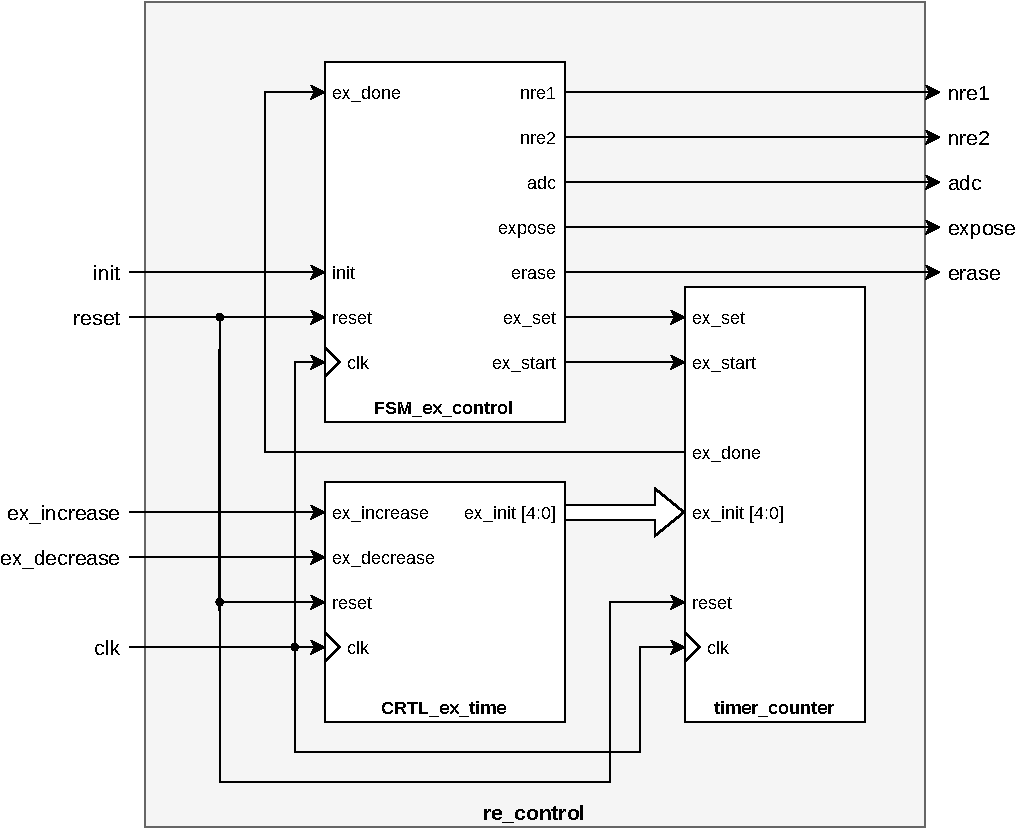
\includegraphics[width=.9\textwidth]{Images/Block_diagrams/re_control_block.pdf}
    \caption{Block diagram for the top level digital block. Top level contain the three smaller blocks that actually contain the logic.}
    \label{fig:pros:dig:block}
\end{figure}

There are three logic blocks inside the top level block, \texttt{FSM\_ex\_control}, \texttt{CTRL\_ex\_time} and\\ \texttt{timer\_counter}. 
The main control block and FSM is the \texttt{FSM\_ex\_control} block.
The FSM is implemented with a clock triggered switch statement. 
Each time this is triggered, it checks the current state, and operates according to what the state should do. 
When the FSM is in the EXPOSURE state, the two other blocks are used. 
The \texttt{CTRL\_ex\_time} block, only has a counter with how many milliseconds the exposure should last.
While \texttt{timer\_counter} uses a downward counting counter, to keep track of the exposure time. 
When done the \texttt{ex\_done} flag is set high, so that the FSM can continue to the next state which is READOUT.

In READOUT there is another smaller and simpler FSM, just to clock out the various control signals for the pixels and pixel array. 

When readout is done, the FSM returns back to the IDLE state.

The purpose of the ILLEGAL state is to ensure that all the control signals and the two other blocks are set to their proper stationary state. 
For instance if you are in the middle of an exposure, and suddenly trigging \texttt{reset} to 1. 
The ILLEGAL state will then ensure that the camera FSM can start properly from IDLE.


